\section{Dynamische Programmanalysen und Testen}
The older I get, the more aggressive I get about testing. I like Kent Beck’s rule of thumb that a developer should write at least as much test code as production code. Testing should be a continuous process. No code should be written until you know how to test it. Once you have written it, write the tests for it. Until the test works, you cannot claim to have finished writing the code.

\subsection{Einleitung}

\begin{figure}[h]
	\centering
	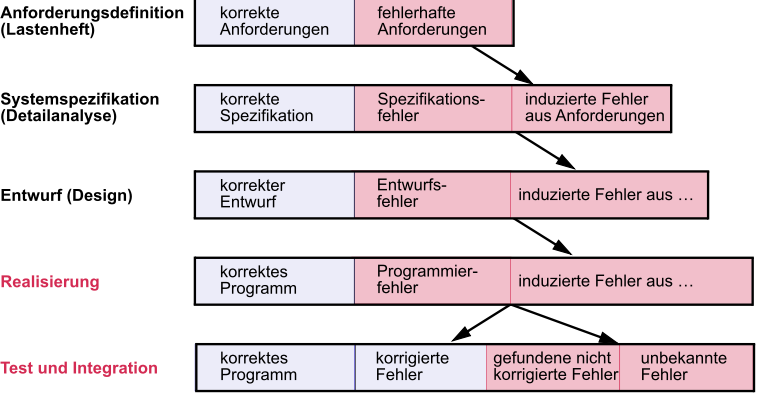
\includegraphics[width=0.85\textwidth]{4_1}
\end{figure}

\paragraph{Fehlerzustand, Fehlerwirkung und Fehlhandlung (DIN 66271):}

\begin{itemize}
	\item \textbf{Fehlerzustand (fault) - direkt erkennbar durch statische Tests: }
	\begin{itemize}
		\item inkorrektes Teilprogramm, inkorrekte Anweisung oder Datendefinition, die Ursache für Fehlerwirkung ist
		\item Zustand eines Softwareprodukts oder einer seiner Komponenten, der unter spezifischen Bedingungen eine geforderte Funktion beeinträchtigen kann
	\end{itemize}
	\item \textbf{Fehlerwirkung (failure) - direkt erkennbar durch dynamische Tests: }
	\begin{itemize}
		\item Wirkung eines Fehlerzustandes, die bei der Ausführung des Testobjektes nach ''außen'' in Erscheinung tritt
		\item Abweichung zwischen spezifiziertem Soll-Wert (Anforderungsdefinition) und beobachtetem Ist-Wert (bzw. Soll- und Ist-Verhalten)
	\end{itemize}
	\item \textbf{Fehlhandlung (error): }
	\begin{itemize}
		\item menschliche Handlung (des Entwicklers), die zu einem Fehlerzustand in der Software führt
		\item \textbf{NICHT einbezogen:} menschliche Handlung eines Anwenders, die ein unerwünschtes Ergebnis zur Folge hat
	\end{itemize}
\end{itemize}

\paragraph{Ursachenkette für Fehler (in Anlehnung an DIN 66271):}

\begin{itemize}
	\item jeder Fehler (\textbf{fault}) oder Mangel ist seit dem Zeitpunkt der Entwicklung in der Software vorhanden - Software nützt sich nicht ab
	\item er ist aufgrund des fehlerhaften Verhaltens (\textbf{error}) eines Entwicklers entstanden (und wegen mangelhafter Qualitätssicherungsmaßnahmen nicht entdeckt worden)
	\item ein Softwarefehler kommt nur bei der Ausführung der Software als Fehlerwirkung (\textbf{failure}) zum Tragen und führt dann zu einer ggf. sichtbaren Abweichung des tatsächlichen Programmverhaltens vom gewünschten Programmverhalten
	\item Fehler in einem Programm können durch andere Fehler \textbf{maskiert} werden und kommen somit ggf. nie zum Tragen (bis diese anderen Fehler behoben sind)
\end{itemize}

\paragraph{Validation und Verifikation (durch dynamische Tests):}
\begin{itemize}
	\item \textbf{Validation von Software: }
	\begin{itemize}
		\item Prüfung, ob die Software das vom Anwender „wirklich“ gewünschte Verhalten zeigt (in einem bestimmten Anwendungsszenario)
		\item Haben wir das richtige Softwaresystem realisiert?
	\end{itemize}
	\item \textbf{Verifikation von Software: }
	\begin{itemize}
		\item Prüfung, ob die Implementierung der Software die Anforderungen erfüllt, die vorab (vertraglich) festgelegt wurden
		\item Haben wir das Softwaresystem richtig realisiert?
	\end{itemize}
\end{itemize}
\textbf{Achtung:} Eine ''richtig realisierte'' = korrekte Software (erfüllt die spezifizierten Anforderungen) 
muss noch lange nicht das ''wirklich'' gewünschte Verhalten zeigen!

\paragraph{Typische Programmierfehler nach [BP84]:}

\begin{itemize}
	\item \textbf{Berechnungsfehler}: Komponente berechnet falsche Funktion
	\begin{itemize}
		\item z.B. Konvertierungsfehler in Fortran bei Variablen, die mit I, J oder K anfangen und damit implizit als Integer deklariert sind
	\end{itemize}
	\item \textbf{Schnittstellenfehler}: Inkonsistenz (bezüglich erwarteter Funktionsweise) zwischen Aufrufsstelle und Deklaration
	\begin{itemize}
		\item Übergabe falscher Parameter, Vertauschen von Parametern
		\item Verletzung der Randbedingungen, unter denen aufgerufene Komponente funktioniert
	\end{itemize}
	\item \textbf{Kontrollflussfehler}: Ausführung eines falschen Programmpfades 
	\begin{itemize}
		\item Vertauschung von Anweisungen
		\item falsche Kontrollbedingung (z.B. ''kleiner'' statt ''kleiner gleich''), ''off by one'': Schleife wird einmal zuwenig oder zu oft durchlaufen
	\end{itemize}
	\item \textbf{Datenflussfehler}: falscher Zugriff auf Variablen und Datenstrukturen
	\begin{itemize}
		\item Variable wird nicht initialisiert (Initialisierungsfehler)
		\item falsche Arrayindizierung
		\item Zuweisung an falsche Variable
		\item Zugriff auf Nil-Pointer oder bereits freigegebenes Objekt
		\item Objekt wird nicht freigegeben
	\end{itemize}
	\item \textbf{Zeitfehler}: gefordertes Zeitverhalten wird nicht eingehalten
	\begin{itemize}
		\item Implementierung ist nicht effizient genug
		\item wichtige Interrupts werden zu lange blockiert
	\end{itemize}
	\item \textbf{Redefinitionsfehler:} geerbte Operation wird nicht semantikerhaltend redefiniert
	\begin{itemize}
		\item ein ''Nutzer'' der Oberklasse geht von Eigenschaften der aufgerufenen Operation aus, die Redefinition in Unterklasse nicht (mehr) erfüllt
	\end{itemize}
\end{itemize}

\paragraph{Was wird also getestet:}
Testverfahren für Softwarekomponenten (Operation, Klasse, Modul/Paket, System) können danach klassifiziert werden, was getestet wird:
\begin{itemize}
	\item \textbf{Funktionalitätstest}: das Ein-/Ausgabeverhalten der Software; das steht beim Testen (zunächst) stark im Vordergrund
	\item \textbf{Benutzbarkeitstest}: es geht um die „gute“ Gestaltung der Benutzeroberfläche; schwieriges Thema, das hier nicht weiter vertieft wird
	\item \textbf{Performanztest}: Laufzeitverhalten und Speicherplatzverbrauch einer Komponente werden gemessen und dabei oft durchlaufene ineffiziente Programmteile oder Speicherlecks identifiziert
	\item \textbf{Lasttest}: die Komponente wird mit schrittweise zunehmender Systemlast \textbf{innerhalb des zugelassenen/spezifizierten Bereiches} (für Eingabedaten) getestet  
	\item \textbf{Stresstest}: die Systemlast wird solange erhöht, bis sie \textbf{außerhalb des zugelassenen/spezifizierten Bereiches} (für Eingabedaten) liegt; damit wird das Verhalten 
	des Systems unter Überlast beobachtet
\end{itemize}

\paragraph{Wie wird getestet - Aufbau eines Testrahmens}

\begin{figure}[h]
	\centering
	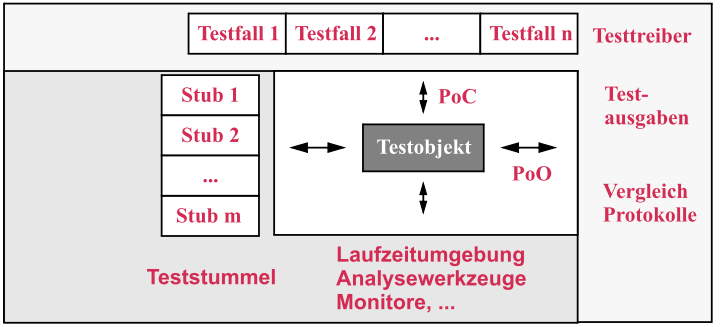
\includegraphics[width=0.85\textwidth]{4_1_1}
\end{figure}

\begin{itemize}
	\item \textbf{Point of Control (PoC): }
	\begin{itemize}
		\item Schnittstelle, über die Testobjekt mit Testdaten versorgt wird
	\end{itemize}
	\item \textbf{Point of Observation (PoO)}
	\begin{itemize}
		\item Schnittstelle, über die Reaktionen/Ausgaben des Testobjekts beobachtet werden
	\end{itemize}
\end{itemize}

\paragraph{Wie wird getestet - Arten von Testverfahren:}

\begin{itemize}
	\item \textbf{Funktionstest}(black box test): die interne Struktur der Komponente wird nicht betrachtet; getestet wird Ein-/Ausgabeverhalten gegen Spezifikation (informell oder formal);
	\item \textbf{Strukturtest}  (white box test): interne Struktur der Komponente wird zur Testplanung und -Überwachung herangezogen:
	\begin{itemize}
		\item Kontrollflussgraph
		\item Datenflussgraph
		\item Automaten
	\end{itemize}
	\item \textbf{Diversifikationstest} Verhalten einer Komponentenversion wird mit Verhalten anderer Komponentenversionen verglichen
\end{itemize}

\paragraph{Diversifikationstestverfahren:}

Das Verhalten verschiedener Varianten eines Programms wird verglichen
\begin{itemize}
	\item \textbf{Mutationstestverfahren}: ein Programm wird absichtlich durch Transformationen verändert und damit in aller Regel mit Fehlern versehen
	\begin{itemize}
		\item Einbau von Fehlern lässt sich (mehr oder weniger) automatisieren
		\item eingebaute Fehler entsprechen oft nicht tatsächlich gemachten Fehlern
		\item eingebaute Fehler stören Suche nach echten Fehlern
	\end{itemize}
	\item \textbf{N-Versionen-Programmierung}: verschiedene Versionen eines Programms werden völlig unabhängig voneinander entwickelt
	\begin{itemize}
		\item sehr aufwändig, da man mehrere Entwicklerteams braucht (und gegebenfalls sogar Hardware mehrfach beschaffen muß)
		\item Fehler der verschiedenen Teams nicht unabhängig voneinander (z.B. haben alle Versionen dieselben Anforderungsdefinitionsfehlern)
	\end{itemize}
\end{itemize}

\paragraph{Mutationstestverfahren:}

\textbf{Erzeugung von Mutationen durch:} \\
Vertauschen von Anweisungsfolgen, Umdrehen von Kontrollflussbedingungen, Löschen von Zuweisungen, Ändern von Konstanten, …
\\
\\
\textbf{Zielsetzungen:}
\begin{itemize}
	\item I\textbf{dentifikation fehlender Testfälle}: für jeden Mutanten sollte mindestens ein Testfall existieren, der Original und Mutant unterscheiden kann
	\item \textbf{Eliminination nutzloser Testfälle}: Gruppe von Testfällen verhält sich bezüglich der Erkennung von Mutanten völlig gleich
	\item Schätzung der Restfehlermenge RF: RF \~ GF*(M/GM-1) \\
	\textbf{Annahme:}  GF/F ~ GM/M (Korrelation gilt allenfalls für bestimmte Fehler) \\
	mit:
	\begin{itemize}
		\item GM = Anzahl gefundener eingebauter Fehler (Mutationen)
		\item M  = Gesamtzahl absichtlich eingebauter Fehler
		\item GF  = Anzahl gefundener echter Fehler
		\item F = Gesamtzahl echter Fehler = GF + RF
	\end{itemize}
\end{itemize}

\paragraph{N-Versionen-Programmierung (Back-to-Back-Testing):}

\textbf{Zielsetzungen:}
\begin{itemize}
	\item eine Version kann als Orakel für die Korrektheit der Ausgaben einer anderen Version herangezogen werden (geht ab 2 Versionen)
	\item Robustheit der ausgelieferten Software kann erhöht werden durch gleichzeitige Berechnung eines benötigten Ergebnisses durch mehrere Versionen einer Software
	\item Liefern verschiedene Versionen unterschiedliche Ergebnisse, so wird Mehrheitsentscheidung verwendet (geht ab 3 Versionen)
\end{itemize}
\textbf{Probleme:}
\begin{itemize}
	\item N Versionen enthalten mehr Fehler als eine Version: falsche Versionen können richtige überstimmen oder gemeinsame Ressourcen blockieren
	\item Fehler verschiedener Versionen sind nicht immer unabhängig voneinander: Fehler aus der Anforderungsdefinition oder typische Programmiersprachenfehler oder falsche Algorithmen können alle Versionen enthalten
\end{itemize}

\paragraph{Exkurs zur Berechnung von Ausfallwahrscheinlichkeiten:}

Für die Berechnung der Ausfallwahrscheinlichkeit eines (Software-)Systems wird der innere Aufbau des Systems wie folgt als ein gerichteter (Kontrollfluss-)Graph bzw. Abhängigkeitsgraph $S=(N,E,n_{start},n_{final})$ dargestellt:
\begin{itemize}
	\item die Knoten N sind die \textbf{Komponenten}, aus denen das System besteht
	\item die Kanten E beschreiben \textbf{Berechnungsabhängigkeiten} bzw. -pfade zwischen den Komponenten des Systems
	\item eine zusätzlich gegebene Funktion A: N ->[0..1] legt für jede Komponente n deren \textbf{Ausfallwahrscheinlichkeit} A(n) fest, die unabhängig von den Ausfallwahrscheinlichkeiten anderer Komponenten sein soll
\end{itemize}
Ein solches System gilt im einfachsten Fall als genau dann \textbf{ausgefallen}, sobald es keinen Pfad von $n_{start}$ nach $n_{final}$ gibt, af dem keine Komponente ausgefallen ist.

\paragraph{Einfache Rechenregeln für System-Ausfallwahrscheinlichkeit:}

Eine \textbf{''Parallelschaltung''} zweier unabhängiger Komponenten $n_{1}$  und $n_{2}$  fällt dann aus, wenn beide Komponenten ausfallen. Das Bild rechts 
zeigt die Ersetzung der Parallelschaltung der beiden Komponenten $n_{1}$  und $n_{2}$  durch eine Komponente n mit gleicher Ausfallwahrscheinlichkeit.
\\
\\
Eine \textbf{''Reihenschaltung''} zweier unabhängiger Komponenten $n_{1}$  und $n_{2}$  ist dann nicht ausgefallen, wenn beide Komponenten nicht ausgefallen sind. Das Bild rechts zeigt die Ersetzung der Reihenschaltung von $n_{1}$  und $n_{2}$  durch eine Komponente n mit gleicher Ausfallwahrscheinlichkeit.

\paragraph{Rekursive Rechenregel für System-Ausfallwahrscheinlichkeit}

Die Berechnung der Ausfallwahrscheinlichkeit eines Systems S lässt sich bei Fokus auf den Status einer bestimmten Komponente n in zwei Fälle zerlegen:
\begin{enumerate}
	\item Berechnung der Ausfallwahrscheinlichkeit von S unter der Annahme, dass die \textbf{Komponente n ausgefallen} ist $=A(S)_{n ist ausgefallen}$; n ist ausgefallen  ; dabei sei A(n) die Wahrscheinlichkeit, dass Komponente n ausgefallen ist.
	\item Berechnung der Ausfallwahrscheinlichkeit von S unter der Annahme, dass die \textbf{Komponente n nicht ausgefallen} ist $=A(S)_{n ist nicht ausgefallen}$; dabei sei 1-A(n) die Wahrscheinlichkeit, dass Komponente n nicht ausgefallen ist.
\end{enumerate}
Damit ergibt sich 
\begin{equation}
	A(S)=A(n) \cdot A(s)_{n ist ausgefallen} + (a-A(n)) \cdot A(S)_{n ist nicht ausgefallen}
\end{equation}
Als Komponente n für die Fallunterscheidung wählt man geschickterweise eine Komponente, die ansonsten die vollständige Dekomposition des betrachteten Graphen in  einfach zu behandelnde Serien- und Parallelschaltungen verhindert. Die Berechnung erfolgt durch die Berechnung der Ausfallwahrscheinlichkeiten zweier ''Ersatzschaltbilder'':
\begin{enumerate}
	\item $A(S)_{n ist ausgefallen}=A(S1)$
	\item $A(S)_{n ist nicht ausgefallen}=A(S2)$
\end{enumerate}

\begin{figure}[h]
	\centering
	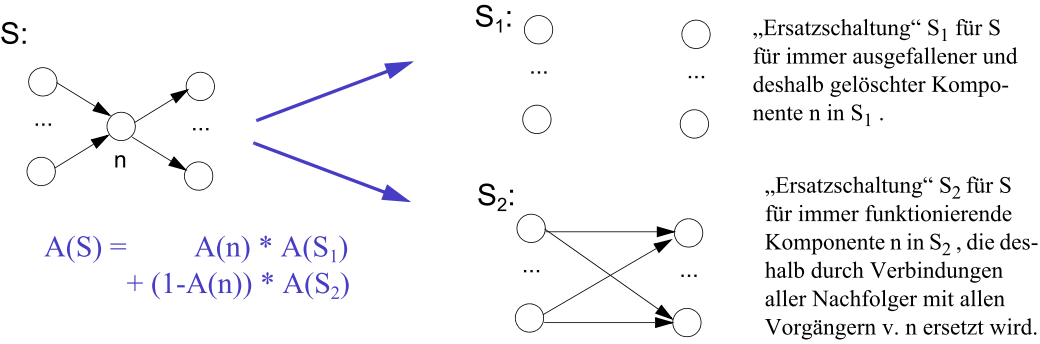
\includegraphics[width=0.85\textwidth]{4_1_2}
\end{figure}

In einigen Fällen muss man auch Komponenten behandeln, die nur dann ''funktionieren'', wenn alle ihre Eingänge korrekte Eingaben erhalten (und damit alle ihre Vorgängerkomponenten nicht ausgefallen sind). Wenn bei einer solchen Komponente eine Vorgängerkomponente ausfällt, fällt die Komponente selbst auch aus.

\paragraph{Alternative Berechnung der Ausfallwahrscheinlichkeit von n Versionen:}

n parallel geschaltete Versionen enthalten in etwa n-mal so viele Fehler wie eine Version, aber falls Wahrscheinlichkeit A für fehlerhafte Arbeitsweise einer Version v unabhängig vom Ausfall anderer Versionen ist, dann gilt:
\begin{itemize}
	\item Richtiges Ergebnis werde berechnet, solange höchstens $\lfloor(n+1)/2\rfloor$ Versionen fehlerhaft arbeiten (n ist sinnvoller Weise ungerade Zahl; ansonsten abrunden)
	\item Wahrscheinlichkeit für gleichzeitigen Ausfall von k unabhängigen Versionen: \\
	$\left(
	\begin{array}{c}
	n \\
	k
	\end{array} x A^k x (1-A)^{(n-k)} =
	\frac{\prod_{i=n-k+1}^{v}i}{\prod_{i=1}^{k}i} x A^k x (1-A)^{(n-k)}
	\right)$
	\item Wahrscheinlichkeit für \textbf{Ausfall des Gesamtsystems} mit n Versionen (bei n=3: Wahrscheinlichkeit für Ausfall von 2 oder 3 Versionen): \\
	$\sum_{\lfloor(n+1)/2\rfloor}^{n\left(
		\begin{array}{c}
		n \\
		k
		\end{array} \right) x A^k x (1-A)^{(n-k)}}$ 
\end{itemize}


\begin{figure}[h]
	\centering
	\caption{Der Testprozess als Bestandteil des Softwareentwicklungsprozesses}
	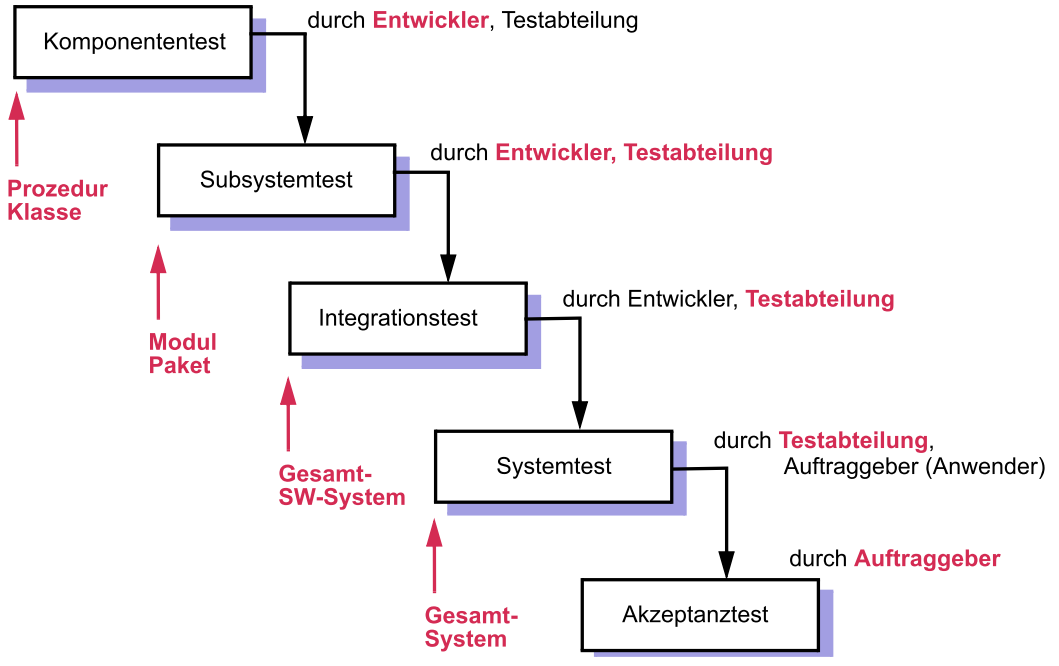
\includegraphics[width=0.85\textwidth]{4_1_3}
\end{figure}


\begin{figure}[h]
	\centering
	\caption{Der Testprozess als Bestandteil des Softwareentwicklungsprozesses}
	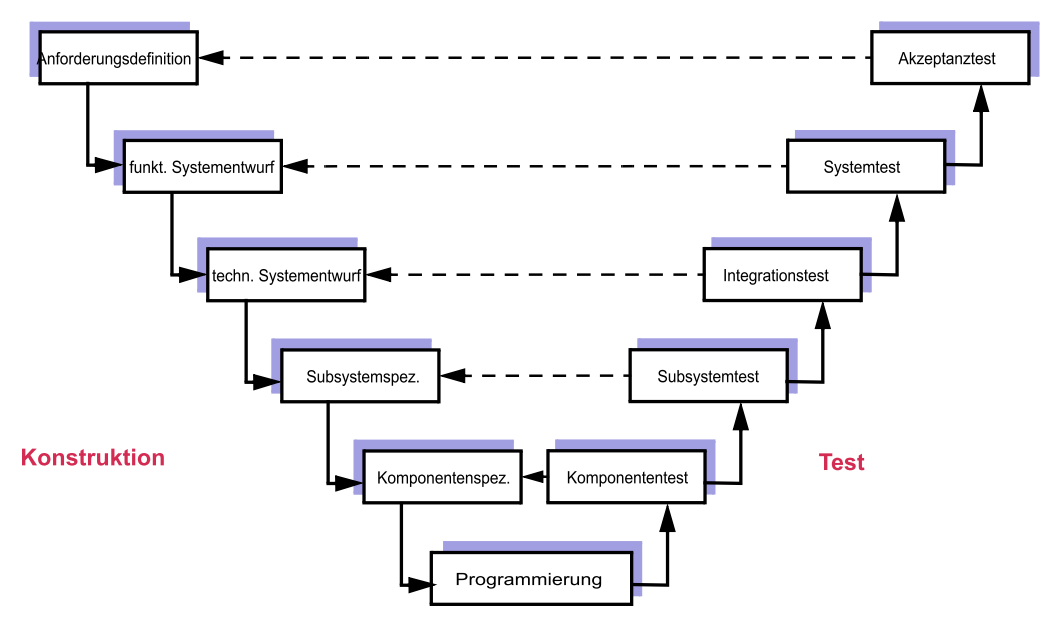
\includegraphics[width=0.85\textwidth]{4_1_4}
\end{figure}

\paragraph{Komponententest (Unit-Test) und Subsystemtest:}

\begin{itemize}
	\item jeweils ein \textbf{einzelner Softwarebaustein} wird überprüft, isoliert von anderen Softwarebausteinen des Systems
	\item die betrachtete Komponente (Unit) kann eine Klasse, Paket (Modul) sein
	\item \textbf{Subsystemtest} kann als Test einer besonders großen Komponente aufgefasst werden
	\item getestet wird gegen die Spezifikation der Schnittstelle der Komponente, dabei betrachtet werden funktionales Verhalten, Robustheit, Effizienz, ...
	\item Testziele sind das Aufdecken von Berechnungsfehlern, Kontrollflussfehlern, ...
	\item getestet wird in jedem Fall die Komponente für sich mit
	\begin{itemize}
		\item \textbf{Teststummel} (Platzhalter, Dummies, Stubs) für benötigte Dienste anderer Komponenten
		\item \textbf{Testtreibern}(Driver) für den (automatisierten) Test der Schnittstelle (für Eingabe von Parametern, Ausgabe von Parametern, ... )
	\end{itemize}
\end{itemize}

\paragraph{Integrationtest:}

\begin{itemize}
	\item das gesamte Software-System (oder ein abgeschlossenes Teilsystem) wird getestet; Schwerpunkt liegt dabei auf Test des \textbf{Zusammenspiels} der Einzelkomponenten
	\item normalerweise wird vorausgesetzt, dass Einzelkomponenten vorab bereits getestet wurden
	\item auch hier müssen wieder \textbf{Testtreiber} (Testwerkzeuge) verwendet werden, die die zu testende Komponente aufrufen bzw. steuern
	\item auf \textbf{Teststummel} kann meist verzichtet werden, da alle benötigten Teilsysteme zusammen getestet werden
	\item \textbf{Testziel} ist vor allem das Aufdecken von \textbf{Schnittstellenfehlern} und insbesondere Fehler beim Austausch von Daten
\end{itemize}

\paragraph{Gängige Integrationsteststrategien:}
\begin{itemize}
	\item \textbf{''Big Bang''-Strategie}: alle Teile sofort integrieren und nur als Gesamtheit testen
	\begin{itemize}
		\item Lokalisierung von Fehlern schwierig
		\item Arbeitsteilung kaum möglich
		\item Testen beginnt zu spät
	\end{itemize}
	\item \textbf{''Top-down''-Testverfahren:} zuerst A mit Dummies für B,C und D; dann B mit Dummies für E und F,...
	\begin{itemize}
		\item Erstellung ''vernünftiger'' Dummies schwierig
		\item Test der Basisschicht sehr spät
	\end{itemize}
	\item \textbf{''Bottom-Up''-Testverfahren:} zuerst E,F,G und H mit Testtreibern, die Einbindung in B,C und D simulieren, dann B,C und D mit Testtreiber...
	\begin{itemize}
		\item Test des Gesamtverhaltens des Systems gegen Lastenheft erst am Ende
		\item Designfehler und Effizienzprobleme werden oft erst spät entdeckt
	\end{itemize}
	\item \textbf{Ad-Hoc-Integration:} die Komponenten werden in der (zufälligen) Reihenfolge ihrer Fertigstellung integriert und getestet
	\item \textbf{Backbone-Integration (Inkrementelle Vorgehensweise):} zunächst wird Grundgerüst erstellt, weitere Komponenten werden stückweise hinzugefügt
	\begin{itemize}
		\item wie erstellt und testet man Grundgerüst (z.B. Top-Down-Testen)
		\item Hinzufügen von Komponenten kann bisherige Testergebnisse entwerten
	\end{itemize}
	\item \textbf{Regressionstest (für inkrementelle Vorgehensweise):} da Änderungen neue Fehlerzustände in bereits getesteten Funktionen verursachen (oder bislang maskierte Fehlerzustände sichtbar machen) können werden
	\begin{itemize}
		\item möglichst viele Tests automatisiert
		\item bei jeder Änderung werden alle vorhandenen Tests durchgeführt
		\item neue Testergebnisse mit alten Testergebnissen verglichen
	\end{itemize}
\end{itemize}


\begin{figure}[h]
	\centering
	\caption{Gängige Integrationsteststrategien}
	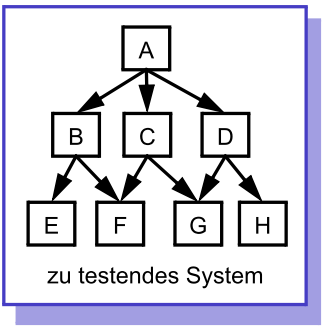
\includegraphics[width=0.3\textwidth]{4_1_5}
\end{figure}

\paragraph{Systemtest - grundsätzliche Vorgehensweise:}
\begin{itemize}
	\item Nach abgeschlossenem Integrationstest und vor dem Abnahmetest erfolgt der Systemtest beim Softwareentwickler durch Kunden $\alpha-Test$
	\item Variante: Systemtests bei ausgewählten Pilotkunden vor Ort $\beta-Test$
	\item Systemtest überprüft aus der \textbf{Sicht des Kunden}, ob das Gesamtprodukt die an es gestellten Anforderungen erfüllt (nicht mehr aus Sicht des Entwicklers)
	\item anstelle von Testtreibern und Teststummeln kommen nun soweit möglich immer die realen (Hardware-)Komponenten zum Einsatz
	\item Systemtest sollte nicht beim Kunden in der Produktionsumgebung stattfinden, sondern in möglichst realitätsnaher Testumgebung durchgeführt werden
	\item beim Test sollten die \textbf{tatsächlichen Geschäftsprozesse} beim Kunden berücksichtigt werden, in das getestete System eingebettet wird
	\item dabei durchgeführt werden: Volumen- bzw. Lasttests (große Datenmengen), Stresstests (Überlastung), Test auf Sicherheit, Stabilität, Robustheit, ...
\end{itemize}

\paragraph{Systemtest - nichtfunktionale Anforderungen:}
\begin{itemize}
	\item  \textbf{Lasttest}: Messung des Systemverhaltens bei steigender Systemlast
	\item \textbf{Performanztest}: Messung der Verarbeitungsgeschwindigkeit unter bestimmten Randbedingungen
	\item \textbf{Kompatibilität}: Verträglichkeit mit vorhandenen anderen Systemen, korrekter Import und Export externer Datenbestände, ...
	\item \textbf{Benutzungsfreundlichkeit}: übersichtliche Oberfläche, verständliche Fehlermeldungen, Hilfetexte, ... - für die jeweilige Benutzergruppe
	\item \textbf{Benutzerdokumentation}: Vollständigkeit, Verständlichkeit, ...
	\item \textbf{Änderbarkeit, Wartbarkeit}: modulare Systemstruktur, verständliche Entwicklerdokumentation, ...
	\item ...
\end{itemize}

\paragraph{Akzeptanztest (Abnahmetest):}
\begin{itemize}
	\item Es handelt sich um eine \textbf{spezielle Form des Systemtests}
	\begin{itemize}
		\item der Kunde ist mit einbezogen bzw. führt den Test durch
		\item der Test findet beim Kunden, aber in Testumgebung statt (Test in Produktionsumgebung zu gefährlich)
	\end{itemize}
	\item auf Basis des Abnahmetests entscheidet Kunde, ob das bestellte Softwaresystem \textbf{mangelfrei} ist und die im Lastenheft festgelegten Anforderungen erfüllt
	\item die durchgeführten Testfälle sollten bereits im \textbf{Vertrag} mit dem Kunden spezifiziert sein
	\item im Rahmen des Abnahmetests wird geprüft, ob System von allen relevanten Anwendergruppen \textbf{akzeptiert} wird
	\item im Rahmen von sogenannten \textbf{Feldtests} wird darüber hinaus ggf. das System in verschiedenen Produktionsumgebungen getestet
\end{itemize}

\paragraph{Testen, testen, ... - wann ist Schluss damit?}
\begin{itemize}
	\item \textbf{nie} - nach jeder Programmänderung wird eine große Anzahl von Testfällen automatisch ausgeführt (siehe Regressionstest)
	\item Testbudget verbraucht bzw. Auslieferungszeitpunkt für Software erreicht (der Kunde testet unfreiwillig weiter ... )
	\item je Testfall (Zeiteinheit) gefundene Fehlerzahl sinkt unter gegebene Grenze (in der Hoffnung, dass die Anzahl der im Programm verbliebenen Fehler mit der Anzahl der pro Zeiteinheit gefundenen Fehler korreliert)
	\item n\% absichtlich von einer Gruppe implantierter Fehler (seeded bugs) wurden von Testgruppe gefunden (siehe auch Mutationstestverfahren)
	\item gemäß systematischen Verfahren werden aus allen möglichen Eingabedatenkombinationen typische Repräsentanten ausgewählt und genau diese getestet
	\item Testfälle decken hinreichend viele (relevante) Programmdurchläufe ab
\end{itemize}

\paragraph{Die sieben Grundsätze des Testens nach [SL19]:}
\begin{enumerate}
	\item Testen zeigt die Anwesenheit von Fehlern (und nie die Abwesenheit)
	\item Vollständiges Testen ist nicht möglich
	\item Mit dem Testen frühzeitig beginnen
	\item Häufung von Fehlern (in bestimmten Programmteilen)
	\item Zunehmende Testresistenz (gegen existierende Tests)
	\item Testen ist abhängig vom Umfeld
	\item \textbf{Trugschluss}: Keine Fehler bedeutet ein brauchbares System
\end{enumerate}

\subsection{Laufzeit- und Speicherplatzverbrauchsmessungen}
Gemeinsame Eigenschaft aller hier vorgestellten Werkzeuge/Verfahren ist:
\begin{itemize}
	\item Objektcode für untersuchte Software wird vor Ausführung ''instrumentiert'' (um zusätzliche Anweisungen ergänzt)
	\item zusätzliche Anweisungen erzeugen während der Ausführung statistische Daten über Laufzeitverhalten, Speicherplatzverbrauch, ...
\end{itemize}


\begin{figure}[h]
	\centering
	\caption{Laufzeit- und Speicherplatzverbrauchsmessungenn}
	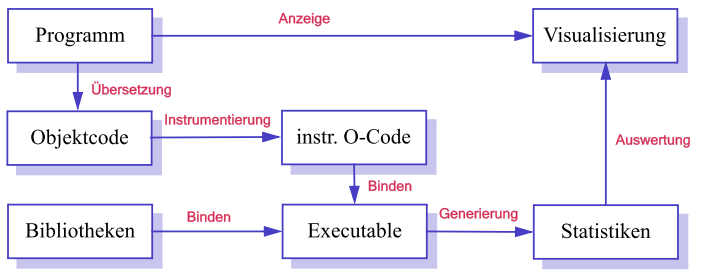
\includegraphics[width=0.85\textwidth]{4_2}
\end{figure}

\paragraph{Untersuchung des Laufzeitverhaltens eines Programms:}
\begin{itemize}
	\item wie oft wird jede Operation aufgerufen (oder Quellcodezeile durchlaufen)
	\item welche Operation ruft wie oft welche andere Operation (\textbf{descendants}) auf oder von welchen Operationen (\textbf{callers}) wird ein Programm wie oft gerufen
	\item wieviel Prozent der Gesamtlaufzeit wird mit Ausführung einer bestimmten Operation verbracht (ggf. aufgeteilt nach callers und descendants)
	\item ...
\end{itemize}

\paragraph{Nutzen der ermittelten Daten:}
\begin{itemize}
	\item  Operationen, die am meisten Laufzeit in Anspruch nehmen, können leicht identifiziert (und optimiert) werden
	\item tatsächliche Aufrufabhängigkeiten werden sofort sichtbar
	\item ...
\end{itemize}

\paragraph{Untersuchung des Speicherplatzverhaltens eines Programms:}
\begin{itemize}
	\item welche Operationen fordern wieviel Speicherplatz an (geben ihn frei)
	\item wo wird Freigabe von Speicherplatz vermutlich bzw. bestimmt vergessen (memory leak = Speicherloch):
	\begin{itemize}
		\item bestimmt vergessen: Objekt lebt noch, kann aber nicht mehr erreicht werden (Garbage Collector von Java würde es entsorgen)
		\item vermutlich vergessen: Objekt lebt noch und ist erreichbar, wird aber nicht mehr benutzt (Garbage Collector von Java kann es nicht freigeben)
	\end{itemize}
	\item wo wird auf bereits freigegebenen Speicherplatz zugegriffen (nur für C++) bzw. wo wird Speicherplatz mehrfach freigegeben (nur für C++)
	\item wo wird auf nicht initialisierten Speicherplatz zugegriffen; anders als bei der statischen Programmanalyse wird für jede Feldkomponente (Speicherzelle) getrennt Buch darüber geführt 
	\item wo finden Zugriffe jenseits der Grenzen von Arrays statt (Laufzeitfehler in guter Programmiersprache)
\end{itemize}

\subsection{Funktionsorientierte Testverfahren (Blackbox)}

Sie testen Implementierung gegen ihre Spezifikation und lassen die interne Programmstruktur unberücksichtigt (Programm wird als ''Black-Box'' behandelt):
\begin{itemize}
	\item für \textbf{Abnahmetest} ohne Kenntnis des Quellcodes geeignet
	\item setzt (eigentlich) vollständige und widerspruchsfreie \textbf{Spezifikation} voraus (zur Auswahl von Testdaten und Interpretation von Testergebnissen)
	\item \textbf{repräsentative Eingabewerte} müssen ausgewählt werden (man kann im allgemeinen nicht alle Eingabekombinationen testen)
	\item man braucht ''Orakel'' für Überprüfung der Korrektheit der Ausgaben (braucht man allerdings bei allen Testverfahren)
\end{itemize}

Eingaben -> Testobjekt -> Ausgaben -> Orakel -> Ausgabe ok?

\paragraph{Kriterien für die Auswahl von Testdaten:}

An der Spezifikation orientierte \textbf{Äquivalenzklassenbildung}, so dass für alle Werte einer Äquivalenzklasse (Eingabewertklasse) sich das Softwareprodukt ''gleich'' verhält:
\begin{itemize}
	\item Unterteilung in Klassen von Eingabewerten, für die das Programm sich laut Spezifikation gleich verhalten muss
	\item Alle Klassen von Eingabewerten zusammen müssen den ganzen möglichen Eingabewertebereich des betrachteten Programms abdecken
	\item Aus jeder Äquivalenzklasse wird mindestens ein repräsentativer Wert getestet
	\item Unterteilung in gültige und ungültige Eingabewerte (fehlerhafte Eingaben, ... ) wird durchgeführt und später bei der Auswahl von Testwerten berücksichtigt
	\item Oft gibt es auch eine gesonderte Betrachtung von Äquivalenzklassen für besonders ''große'' oder besonders ''kleine'' gültige Eingaben (Lasttest)
	\item Hier nicht mit betrachtet wird die Problematik der Suche nach Eingabewerteklassen, die zu bestimmten (Klassen von) Ausgabewerten führen 
\end{itemize}

\paragraph{Regeln für die Festlegung von Eingabewerteklassen:}
\begin{itemize}
	\item für geordnete Wertebereiche:
	\begin{itemize}
		\item $]uv..ov[$ ist ein offenes Intervall aller Werte zwischen $uv$ und $ov$ ($uv$ und $ov$ selbst gehören nicht dazu)
		\item $[uv..ov]$ ist ein geschlossenes Intervall aller Werte zwischen $uv$ und $ov$ ($uv$ und $ov$ selbst gehören dazu)
		\item Mischformen $]uv...ov]$ und $[uv..ov[$ sind natürlich erlaubt
	\end{itemize}
	\item für ganze Zahlen (Integer):
	\begin{itemize}
		\item $[MinInt..ov]$ für Intervalle mit kleinster darstellbarer Integer-Zahl
		\item $[uv..MaxInt]$ für Intervalle mit größter darstellbarer Integer-Zahl
		\item offene Intervallgrenzen sind natürlich erlaubt
	\end{itemize}
	\item für reelle Zahlen (Float) mit Voraussetzung kleinste/größte Zahl nicht darstellbar:
	\begin{itemize}
		\item $]-\infty..ov]$ oder $]-\infty..ov[$ für nach unten offene Intervalle
		\item $[uv..\infty[$ oder $]uv..\infty$ für nach oben offene Intervalle
		\item alle Mischformen von Intervallen mit festen unteren und oberen Grenzen
	\end{itemize}
	\item für Zeichenketten (String):
	\begin{itemize}
		\item Definition über reguläre Ausdrücke oder Grammatiken
		\item Aufzählung konkreter Werte (siehe nächster Punkt)
	\end{itemize}
	\item für beliebige Wertebereiche:
	\begin{itemize}
		\item {v1 v2 v3 ... vn} für Auswahl von genau n verschiedenen Werten
	\end{itemize}
	\item für zusammengesetzte Wertebereiche:
	\begin{itemize}
		\item Anwendung der obigen Prinzipien auf die einzelnen Wertebereiche
		\item ggf. braucht man noch zusätzliche Einschränkungen (Constraints), die nur bestimmte Wertekombinationen für die Teilkomponenten zulassen
	\end{itemize}
	\item Eingabewerteklassen, die aus genau einem Wert bestehen:
	\begin{itemize}
		\item [v] es ist aber auch die Repräsentation {v} oder v üblich
	\end{itemize}
\end{itemize}

\paragraph{Auswahl von Testdaten aus Eingabewerteklassen:}

\begin{itemize}
	\item aus jeder Eingabewerteklasse wird mindestens ein Wert ausgewählt (Fehler- und Lasttestklassen werden später gesondert behandelt) 
	\item gewählt werden meist nicht nur die Grenzen selbst, sondern auch die um eins größeren und kleineren Werte (siehe ISTQB-Prüfung; im Folgenden werden aus Platzgründen bei den Beispielen aber nur Grenzwerte selbst ausgewählt)
	\item als Intervalle dargestellte Eingabewerteklassen werden oft durch die so genannte \textbf{Grenzwertanalyse} nochmal in Unterklassen/Teilintervalle zerlegt:
	\begin{itemize}
		\item $]uv..ov[$ wird zerlegt $[inc(uv)] ]inc(uv)..dec(ov)[ [dec(ov)]$
		\item $[uv..ov]$ wird zerlegt in $[uv] ]uv..ov[ [ov]$
		\item ...
		\item $inc(uv)$ liefert den nächstgrößeren Wert zu uv
		\item $dec(ov)$ liefert den nächstkleineren Wert zu ov
		\item Achtung: bei Float muss für inc und dec die gewünschte Genauigkeit festgelegt werden, mit der aufeinanderfolgende Werte gewählt werden
	\end{itemize}
\end{itemize}

\paragraph{Zusätzliche Wahl von Testdaten durch Grenzwertanalyse:}

Bilden Eingabewerteklassen einen Bereich (Intervall), so selektiert die Grenzwertanalyse also immer Werte um die Bereichsgrenzen herum:
\begin{itemize}
	\item gewählt werden meist nicht nur die Grenzen selbst, sondern auch die um eins größeren und kleineren Werte (im Folgenden aus Platzgründen weggelassen)
	\item Idee dabei: oft werden Schleifen über Intervallen gebildet, die genau für die Grenzfälle falsch programmiert sind
\end{itemize}

\paragraph{Auswahl von Testeingaben für countVowels (mit Zeichenketten!):}
s = sentence
\begin{itemize}
	\item Klasse 1: s endet nicht mit einem Punkt (oh je, das geht schief)
	\item Klasse 2: s endet mit einem Punkt und enthält keine Vokale
	\begin{itemize}
		\item s besteht nur aus einem Punkt
		\item s besteht aus einem Konsonanten gefolgt von einem Punkt
		\item s enthält sonstige Sonderzeichen
	\end{itemize}
	\item Klasse 3: s endet mit einem Punkt und enthält einen Vokal:
	\begin{itemize}
		\item 3a: s enthält ein a, e, i, o, u
		\item 3b: s enthält ein A, E, I, O, U (oh je, dieser Fall wurde auch vergessen)
	\end{itemize}
	\item Klasse 4: s enthält mehrere Vokale:
	\begin{itemize}
		\item 4a: mehrere gleiche Vokale
		\item 4b: mehrere verschiedene Vokale
	\end{itemize}
	\item Klasse 5: Eingabe ist sehr lang und enthält ganz viele Vokale
\end{itemize}

\paragraph{Weitere Regeln für die Bildung von Äquivalenzklassen bei Intervallen:}
\begin{itemize}
	\item aus Äquivalenzklassen, die (geschlossene) Intervalle sind, werden jeweils die beiden Grenzwerte und ein weiterer Wert (z.B. aus der Mitte des Intervalls) ausgewählt (ohne platzraubenden Zwischenschritt der Zerlegung in drei Teilintervalle)
	\item einelementige Äquivalenzklasse und Wert aus dieser Äquivalenzklasse werden nicht unterschieden, also statt [v] schreiben wir gleich v
	\item reguläre Ausdrücke werden zur Definition v. String-Äquivalenzklassen eingesetzt
\end{itemize}

\paragraph{Grafische Darstellung von Äquivalenzklassen als Klassifikationsbaum:}

\begin{figure}[h]
	\centering
	\caption{Grafische Darstellung von Äquivalenzklassen als Klassifikationsbaum}
	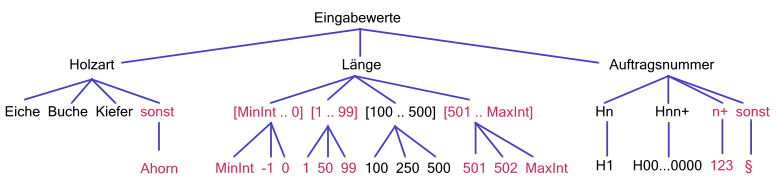
\includegraphics[width=0.85\textwidth]{4_3}
	
\end{figure}
\begin{itemize}
	\item zunächst wird ''Eingabewerte'' in alle Eingabeparameter des Programms zerlegt
	\item zusammengesetzte Eingabeparameter werden weiter zerlegt
	\item schließlich wird der Wertebereich eines atomaren Eingabeparameters betrachtet
	\item der Wertebereich wird in Äquivalenzklassen „ähnlicher“ Werte zerlegt
	\item dabei werden auch nicht erlaubte Eingabewerte (Fehlerklassen) betrachtet
	\item ebenso werden ''extreme'' erlaubte Werte (Lasttestklassen) betrachtet
	\item aus jedem Wertebereich werden Repräsentanten für den Test ausgewählt
\end{itemize}

\paragraph{Unvollständige/fehlerhafte Auswahl von Eingabewertekombinationen:}

\begin{figure}[h]
	\centering
	\caption{Unvollständige/fehlerhafte Auswahl von Eingabewertekombinationen}
	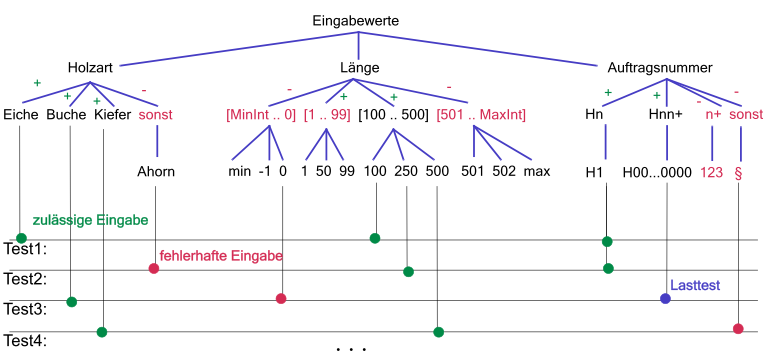
\includegraphics[width=0.85\textwidth]{4_3_1}
\end{figure}

\textbf{Problem:} trotz Bildung von Äquivalenzklassen bleiben (zu) viele mögliche Eingabewertekombinationen (im Beispiel sind 4 * 12 * 4 verschiedene Testläufe möglich).

\paragraph{Heuristiken für die Reduktion möglicher Eingabewertekombinationen:}

\begin{itemize}
	\item aus jeder \textbf{Äquivalenzklasse} wird mindestens einmal ein Wert ausgewählt; es gibt also jeweils mindestens einen Testfall, in dem ein Eingabewert der Äquivalenzklasse verwendet wird (bei Grenzwertanalyse werden drei Werte ausgewählt)
	\item bei \textbf{abhängigen Eingabeparametern} müssen Testfälle für \textbf{alle Kombinationen} ihrer jeweiligen ''normalen'' Äquivalenzklassen aufgestellt werden; Parameter sind abhängig, wenn sie gemeinsam das Verhalten des Programms steuern (und deshalb nicht unabhängig voneinander betrachtet werden können)
	\item der ausgewählte \textbf{Wert} einer \textbf{Fehleräquivalenzklasse} wird in genau einem Testfall verwendet (Fehleräquivalenzklassen sind solche Äquivalenzklassen, die unzulässige Eingabewerte zusammenfassen)
	\item der ausgewählte \textbf{Wert} einer \textbf{Lasttestklasse} wird ebenfalls genau einmal in einem Testfall verwendet  (Lasttestklassen sind solche Äquivalenzklassen, die besonders ''große/lange/...'' zulässige/gültige Eingabewerte zusammenfassen)
	\item hat man mehrere Eingabeparameter, wird \textbf{höchstens einer} mit einem Wert aus einer Fehler- oder Lasttestklasse belegt (verhindert Verdeckung von Fehlern)
\end{itemize}

\paragraph{''Normierter'' Aufbau von Klassifikationsbäumen für Übung/Klausur:}


\begin{enumerate}
	\item Ebene: alle Parameter(-namen) der betrachteten Funktion
	\item Ebene: die Typen bzw. Wertebereiche der Parameter
	\item Ebene: die Zerlegung der Wertebereiche in
	\begin{itemize}
		\item Äquivalenzklassen für erlaubte Werte (mit ''+'' markiert)
		\item Fehleräquivalenzklassen (mit ''-'' markiert)
	\end{itemize}
	\item Ebene:  weitere Zerlegung der Wertebereiche mit Grenzwertanalyseverfahren
	\item Ebene:  konkrete Repräsentanten (Werte) der jeweiligen Äquivalenzklassen
\end{enumerate}

\paragraph{Paarweiser Testansatz (Pairwise Testing):}

Die Praxis zeigt, dass ca. 80\% aller von bestimmten Parameterwertkombinationen ausgelösten Softwarefehler bereits durch Wahl bestimmter Paarkombinationen beobachtet werden können. Also werden beim ''paarweisen'' Testen einer Funktion mit n Parametern nicht alle möglichen Kombinationen überprüft, sondern nur alle paarweisen Kombinationen.

\paragraph{Bewertung der funktionalen Äquivalenzklassenbildung:}

\begin{itemize}
	\item Güte des Verfahrens hängt stark von \textbf{Güte der Spezifikation} ab (Aussagen über erwartete/zulässige Eingabewerte und Ergebnisse)
	\item Verwaltung von Äquivalenzklassen und Auswahl von Testfällen kann durch \textbf{Werkzeugunterstützung} vereinfacht werden
	\item \textbf{ausführbare Modelle} (z.B. in UML erstellt) können bei der Auswahl von Äquivalenzklassen, Testfällen helfen (und als Orakel verwendet werden)
	\item Test von Benutzeroberflächen, zeitlichen Beschränkungen, Speicherplatzbeschränkungen etc. (\textbf{nichtfunktionale Anforderungen}) wird kaum unterstützt
	\item mindestens \textbf{einmalige Ausführung} jeder Programmzeile wird nicht garantiert
	\item Test \textbf{zustandsbasierter Software} (Ausgabeverhalten hängt nicht nur von Eingabe, sondern auch von internem Zustand ab) geht so nicht
	\begin{itemize}
		\item später Spezifikation und Testplanung mit Hilfe von Automaten/Statecharts
		\item Grenzfall zwischen funktionalem und strukturorientiertem Softwaretest
	\end{itemize}
\end{itemize}

\paragraph{Weitere Black-Box-Testverfahren}
\begin{itemize}
	\item \textbf{Erfahrungsbasierte Testverfahren:}
	\begin{itemize}
		\item \textbf{Intuitives Testen (Error Guessing)}: ein Testansatz, bei dem Testfälle auf Basis des Wissens der Tester über frühere Fehler oder allgemeines Wissen über Fehlerwirkungen (irgendwie) abgeleitet werden
		\item \textbf{Exploratives Testen}: ein Testansatz bei dem die Tester, basierend auf ihrem Wissen, der Erkundung des Testobjekts und dem Ergebnis früherer Tests, dynamisch neue Tests entwickeln
		\item \textbf{Checklistenbasiertes Testen}: ein Testansatz bei dem erfahrene Tester eine Liste von Kontrollpunkten (Checkliste) bzw. Regeln oder Kriterien (für das Testobjekt) zur Steuerung des Testprozesses nutzen
	\end{itemize}
	\item \textbf{Zufallstest}: wählt aus Menge der möglichen Werte eines Eingabedatums zufällig Repräsentanten aus (ggf. gemäß bekannter statistischer Verteilung)
	\begin{itemize}
		\item zur Ergänzung gut geeignet, generiert oft ''unerwartete'' Testdaten
	\end{itemize}
	\item \textbf{Smoke-Test:} es wird nur Robustheit des Testobjekts getestet, berechnete Ausgabewerte spielen keine Rolle (auf Tastatur hämmern, ... )
	\item \textbf{Syntax-Test}: ist für Eingabewerte der erlaubte syntaktische Aufbau bekannt (als Grammatik angegeben) kann man daraus systematisch Testfälle generieren; Beispiele:
	\begin{itemize}
		\item syntaktisch korrekte Email-Adressen
		\item zulässige Dateinamen, Verzeichnispfade
		\item Aufbau von Zahlen (Integers, Floats)
		\item ...
	\end{itemize}
	\item \textbf{Zustandsbezogener Test}
	\item \textbf{Ursache-Wirkungs-Graph-Analyse / Entscheidungstabellenbasiertes Testen}
	\item \textbf{Anwendungsfallbasiertes Testen}
\end{itemize}

\paragraph{Ursache-Wirkungs-Graph-Analyse-Verfahren aus [SL19]}

Es handelt sich eigentlich um eine Kombination von zwei Verfahren. Die Basis bilden sogenannte \textbf{''Entscheidungstabellen''}, die Bedingungen an Eingaben und ausgelöste Aktionen eines Systems miteinander verknüpfen. Für die systematische Erstellung einer Entscheidungstabelle wird zunächst ein \textbf{''Ursache-Wirkungs-Graph''} erstellt.
\\
\\
Ein Ursache-Wirkungs-Graph verknüpft Eingaben = \textbf{Ursachen} / Bedingungen mit daraus resultierenden Ausgaben = \textbf{Wirkungen} / Aktionen (durch grafische Darstellung aussagenlogischer Ausdrücke). Die weitere Vorgehensweise ist wie folgt:
\begin{enumerate}
	\item Eine Wirkung wird ausgewählt.
	\item Zu der Wirkung werden alle Kombinationen von Ursachen gesucht, die diese Wirkung hervorrufen.
	\item Für jede gefundene Ursachenkombination wird eine Spalte der Entscheidungstabelle erzeugt.
	\item Die Spalten der Entscheidungstabelle entsprechen Testfällen.
	\item Die Zeilen der Entscheidungstabelle entsprechen allen Ursachen und Wirkungen.
\end{enumerate}

\paragraph{Anwendungsfallbasiertes Testen aus [SL19]:}

Ausgangspunkt für diese Testmethodik ist die Beschreibung von sogenannten \textbf{Anwendungsfällen} (Nutzungsszenarien, Geschäftsvorfällen) eines Systems im Zuge der Anforderungsanalyse. Dabei kommt in der Regel die ''Unified Modeling Language'' (UML) mit ihren Anwendungsfalldiagrammen zum Einsatz.
\begin{itemize}
	\item Anwendungsfalldiagramme erlauben die Beschreibung von Nutzungsszenarien (und damit von Akzeptanztestfällen) auf sehr hohem Abstraktionsniveau sowie die Unterscheidung zwischen normalen Abläufen und Ausnahmen.
	\item Werden einzelne Anwendungsfälle informell / in natürlicher Sprache beschrieben, so werden die dazugehörigen Testfälle \textbf{''manuell''} erstellt.
	\item Werden für die Beschreibung einzelner Anwendungsfälle formalere Notationen wie Sequenz- oder Aktivitätsdiagramme der UML eingesetzt, so können Testwerkzeuge daraus \textbf{automatisch} Code für die Testfallausführung und -bewertung generieren.
\end{itemize}

\paragraph{Bewertung der Ursache-Wirkungs-Graph- und Anwendungsfall-Testens:}
\begin{itemize}
	\item Beide Methoden lassen sich sehr früh im Software-Lebenszyklus einsetzen und eignen sich insbesondere für die Erstellung von Akzeptanztestfällen.
	\item Die Ursache-Wirkungsgraph-Methode erlaubt die bei der Äquivalenzklassenbildung fehlende Verknüpfung von Eingaben und Ausgaben (Ursachen und Wirkungen).
	\item Das Anwendungsfallbasierte Testen erlaubt hingegen nicht nur die Beschreibung einzelner Testvektoren (Eingabewertkombinationen), sondern auch die Spezifikation ganzer Interaktionssequenzen zwischen Umgebung und zu testendem System.
	\item Insbesondere das Anwendungsfallbasierte Testen unterstützt aber nicht die systematische Identifikation fehlender Testfälle (für bestimmte Eingabetestvektoren).
\end{itemize}

\paragraph{Fazit:}
Alle vorgestellten ''Black-Box''-Testmethoden (Funktionsorientierte Testverfahren) besitzen ihre Stärken und Schwächen und ergänzen einander!!!

\subsection{Kontrollflussbasierte Testverfahren (Whitebox)}

\paragraph{Grundideen des kontrollflussbasierten Testens:}
\begin{itemize}
	\item mit im Grunde zunächst beliebigen Verfahren werden \textbf{Testfälle festgelegt}
	\item diese Testfälle werden alle \textbf{ausgeführt} und dabei wird notiert, welche Teile des Programms durchlaufen wurden
	\item es gibt (meist) ein \textbf{Test-Orakel}, dass für jeden ausgeführten Testfall ermittelt, ob die berechnete Ausgabe (Verhalten des Programms) korrekt ist
	\item schließlich wird festgelegt, ob die vorhandenen Testfälle den Kontrollfluss des Programms hinreichend \textbf{überdecken}
	\item ggf. werden solange \textbf{neue Testfälle aufgestellt}, bis hinreichende Überdeckung des Quelltextes (Kontrollflusses) erreicht wurde
	\item ggf. werden \textbf{alte Testfälle gestrichen}, die dieselben Teile des Quelltextes (Kontrollflusses) überdecken
\end{itemize}

\paragraph{Kontrollflusstest - Anweisungsüberdeckung (C0-Test):}
Jeder Knoten des Kontrollflussgraphen muss mindestens einmal ausgeführt werden.
\begin{itemize}
	\item Minimalkriterium, da nicht mal alle Kanten des Kontrollflussgraphen traversiert werden
	\item viele Fehler bleiben unentdeckt
\end{itemize}

\paragraph{Kontrollflusstest - Zweigüberdeckung (C1-Test):}
Jede Kanten des Kontrollflussgraphen muss mindestens einmal ausgeführt werden.
\begin{itemize}
	\item realistisches Minimalkriterium
	\item umfasst Anweisungsüberdeckung
	\item Fehler bei Wiederholung oder anderer Kombination von Zweigen bleiben unentdeckt
\end{itemize}

\paragraph{Kontrollflusstest - Entscheidungs-/Bedingungsüberdeckung:}

Jede Teilbedingung einer Kontrollflussbedingung (z.B. von if- oder while-Anweisung) muss einmal den Wert true und einmal den Wert false annehmen.
\\
\\
\textbf{atomare Bedingungsüberdeckung/-test:}
\begin{itemize}
	\item keine Anforderung an Gesamtbedingung
	\item umfasst nicht mal Anweisungsüberdeckung
\end{itemize}
\textbf{minimale Mehrfachbedingungsüberdeckung/-test:}
\begin{itemize}
\item jede Teil- und Gesamtbedingung ist einmal true und einmal false
\item Orientierung an syntaktischer Struktur von Kontrollflussbedingungen
\item Bedingung umfasst Zweigüberdeckung
\item trotzdem werden viele Bedingungsfehler nicht entdeckt
\end{itemize}

\paragraph{Modifizierter Bedingungsüberdeckungstest (MCDC):}

Der \textbf{modifizierte Bedingungsüberdeckungstest} (Definierter Bedingungstest, Modified Condition Decision Coverage) benötigt wie die bisherigen Überdeckungskriterien eine linear mit der Anzahl der atomaren Teilbedingungen steigende Anzahl von Testfällen. Es werden aber i.A. ''bessere'' Testfälle als bei der minimalen Mehrfachbedingungsüberdeckung gewählt. Die Bedingungen sind:
\begin{itemize}
	\item jeder atomaren Teilbedingung lassen sich zwei Testfälle zuordnen (verschiedene Teilbedingungen dürfen aber die selben Testfälle nutzen)
	\item die Werte aller Teilbedingungen, die für das Gesamtergebnis der Bedingung irrelevant sind und deshalb ggf. wegen ''short circuit''-Evaluation des Compilers nicht ausgewertet werden, werden als irrelevant gekennzeichnet (mit Zeichen ''-'')
	\item die beiden Testfälle zu einer atomaren Teilbedingung setzen diese einmal auf true und einmal auf false und unterscheiden sich nur in der gerade betrachteten atomaren Teilbedingung (irrelevant kann mit true u. false gleichgesetzt werden)
	\item die beiden Testfälle zu einer atomaren Teilbedingung setzen die Gesamtbedingung einmal auf  true und einmal auf false
\end{itemize}

\paragraph{Kontrollflusstest - Pfadüberdeckung (C-unendlich-Test):}
Jeder mögliche Pfad des Kontrollflussgraphen muss einmal durchlaufen werden.
\begin{itemize}
	\item rein theoretisches Kriterium, sobald Programm Schleifen enthält (unendliche viele verschiedene Pfade = Programmdurchläufe möglich)
	\item dient als Vergleichsmaßstab für andere Testverfahren
	\item findet trotzdem nicht alle Fehler (z.B. Berechnungsfehler), da kein erschöpfender Test aller möglichen Eingabewerte
	\item davon abgeleitetete in der Praxis durchführbare Verfahren:
	\begin{itemize}
		\item \textbf{boundary test}: alle Pfade auf denen Schleifen maximal einmal durchlaufen werden (ohne besondere praktische Bedeutung)
		\item \textbf{boundary interior test}: alle Pfade auf denen Schleifen maximal zweimal (in direkter Folge) durchlaufen werden (Achtung: Anzahl Pfade explodiert bei geschachtelten Schleifen und vielen bedingten Anweisungen)
		\item \textbf{modifizierter boundary interior test}: bei geschachtelten Schleifen wird beim Durchlauf einer äußeren Schleife die Anzahl der inneren Schleifendurchläufe nicht unterschieden
	\end{itemize}
\end{itemize}

\paragraph{Bewertung der Kontrollflusstests:}
\begin{itemize}
	\item Anweisungsüberdeckung wird durch RTCA DO-178B-Standard für Software-Anwendungen in der Luftfahrt der \textbf{Kritikalitätsstufe C} gefordert (Software, deren Ausfall zu einer bedeutenden, aber nicht kritischen Fehlfunktion führen kann)
	\item Zweigüberdeckung wird durch RTCA DO-178B-Standard für Software-Anwendungen in der Luftfahrt der \textbf{Kritikalitätsstufe B} gefordert (Software, deren Ausfall zu schwerer aber noch nicht katastrophaler Systemfehlfunktion führen kann)
	\item modifizierte Bedingungsüberdeckung wird durch RTCA DO-178B-Standard für Software-Anwendungen in der Luftfahrt der \textbf{Kritikalitätsstufe A} gefordert (Software, deren Ausfall zu katastrophaler Systemfehlfunktion führen kann)
	\item Zweigüberdeckung sollte für uns Mindestanforderung beim Testen darstellen (Kontrollflussfehler/Bedingungsfehler werden relativ gut gefunden, Datenflussfehler natürlich weniger gut)
	\item Einfache Variante von ''modified boundary interior test'' zur Ergänzung: für jede Schleife gibt es Testfälle/Pfade, die sie gar nicht, genau einmal und (mindestens) zweimal ausführen (die Randbedingung ''alle Pfade'' wird komplett aufgegeben)
\end{itemize}

\subsection{Datenflussbasierte Testverfahren}

Ausgangspunkt ist der Datenflussgraph einer Komponente bzw. der mit Datenflussattributen annotierte Kontrollflussgraph. Bei der Auswahl von Testfällen wird darauf geachtet, dass:
\begin{itemize}
	\item für jede Zuweisung eines Wertes an eine Variable \textbf{mindestens eine} (berechnende, prädikative) Benutzung dieses Wertes getestet wird
	\item oder für jede Zuweisung eines Wertes an eine Variable \textbf{alle} (berechnenden, prädikativen) Benutzungen dieses Wertes getestet werden
\end{itemize}
Die datenflussbasierten Testverfahren haben folgende Vor- und Nachteile:
\begin{itemize}
	\item Vorteile:
	\begin{itemize}
		\item einige Verfahren enthalten die Zweigüberdeckung und finden sowohl Datenflussfehler \textbf{als auch} Kontrollflussfehler
		\item besser geeignet für objektorientierte Programme mit oft einfachem Kontrollfluss aber komplexem Datenfluss
	\end{itemize}
	\item Nachteile:
	\begin{itemize}
		\item es gibt kaum Werkzeuge, die datenflussbasierte Testverfahren unterstützen
	\end{itemize}
\end{itemize}

\paragraph{Kriterien für den Datenflusstest}
\begin{itemize}
	\item \textbf{all-defs-Kriterium}: für jede Definitionsstelle d(x) einer Variablen muss \textbf{ein} definitionsfreier Pfad zu \textbf{einer} Benutzung r(x) existieren (und getestet werden)
	\begin{itemize}
		\item Kriterium kann statisch überprüft werden (entdeckt sinnlose Zuweisungen)
		\item umfasst weder Zweig- noch Anweisungsüberdeckung
		\item bei countVowels reichen Testbeispiele '.' und 'a.'
		\item Verfahren findet einige Berechnungsfehler und kaum Kontrollflussfehler
	\end{itemize}
	\item \textbf{all-p-uses-Kriterium}: für jede Definitionsstelle d(x) wird jeweils ein definitionsfreier Pfad zu \textbf{allen} (erreichbaren) prädikativen Benutzungen p(x) getestet
	\begin{itemize}
		\item entdeckt vor allem Kontrollflussfehler
		\item Berechnungsfehler bleiben oft unentdeckt
		\item \textbf{Anmerkung}: manchmal wird auch Test \textbf{aller} definitionsfreien Pfade von d(x) zu allen p(x) gefordert, die Schleifen nicht mehrfach durchlaufen müssen (dann ist Zweigüberdeckung enthalten)
	\end{itemize}
	\item \textbf{all-c-uses-Kriterium}: für jede Definitionsstelle d(x) wird jeweils \textbf{ein} definitionsfreier Pfad zu \textbf{allen} (erreichbaren) berechnenden Benutzungen c(x) getestet
	\begin{itemize}
		\item entdeckt vor allem Berechnungsfehler
		\item Kontrollflussfehler bleiben oft unentdeckt
		\item lässt sich wegen Bedingungen oft nicht erzwingen
	\end{itemize}
	\item \textbf{all-p-uses-some-c-uses-Kriterium}: für jede Definitionsstelle d(x) wird jeweils \textbf{ein} definitionsfreier Pfad zu \textbf{allen} (erreichbaren) prädikativen Benutzungen p(x) getestet; gibt es keine prädikate Benutzung p(x), so wird wenigstens ein Pfad zu einem berechnenden Zugriff c(x) betrachtet
	\begin{itemize}
		\item entdeckt Kontrollfluss- und auch Berechnungsfehler
		\item umfasst all-def- und all-p-uses-Kriterium
	\end{itemize}
	\item \textbf{all-c-uses-some-p-uses-Kriterium}: … (wird kaum benutzt)
	\item \textbf{all-uses-Kriterium}: all-p-uses- + all-c-uses-Kriterium (wird kaum benutzt)
\end{itemize}

\paragraph{Zusammenfassung des überdeckungsbasierten Testens:}
\begin{itemize}
	\item man wählt ein oder mehrere Überdeckungskriterien aus, die der ''Kritikalität'' der zu entwickelnden Software gerecht werden
	\item Kombination von einem kontrollflussbasierten und einem datenflussbasierten Überdeckungskriterium sinnvoll
	\item man wählt nach beliebiger Methodik initiale Menge von Testfällen aus
	\item dann wird (durch Code-Überdeckungsanalyse-Werkzeug) überprüft, zu wieviel Prozent die gewählten Kriterien erfüllt sind
	\item es werden solange Testfälle hinzugefügt, bis eine vorab festgelegte Prozentzahl für alle gewählten Überdeckungskriterien erfüllt ist (90\% oder ... )
	\item Achtung: 100\% lässt sich in vielen Fällen nicht erreichen (wegen Anomalien
\end{itemize}

\subsection{Testen objektorientierter Programme (zustandsbez. Testen)}
Prinzipiell lassen sich in objektorientierten Sprachen geschriebene Programme wie alle anderen Programme testen. Allerdings gibt es einige Besonderheiten, die das Testen sowohl erschweren als auch erleichtern (können):
\begin{itemize}
	\item Positiv
	\begin{itemize}
		\item die Datenkapselung konzentriert Zugriffsoperationen auf Daten an einer Stelle und erleichtert damit das Testen (Einbau von Konsistenzprüfungen)
		\item die Vererbung mit Wiederverwendung bereits getesteten Codes reduziert die Menge an neu geschriebenem zu testenden Code
	\end{itemize}
	\item Negativ
	\begin{itemize}
		\item die Datenkapselung erschwert das Schreiben von Testtreibern, die auf interne Zustände von Objekten zugreifen müssen
		\item die Vererbung ist eine der Hauptfehlerquellen (falsche Interaktion mit geerbten Code bzw. falsche Redefinition von geerbten Methoden)
		\item dynamisches Binden erschwert die Definition sinnvoller Überdeckungsmetriken ungemein (beim White-Box-Test)
		\item Verhalten von Objektmethoden ist (fast) immer zustandsabhängig
	\end{itemize}
\end{itemize}

\paragraph{Prinzipien beim Tests objektorientierter Programme:}
\begin{itemize}
	\item beim \textbf{''Black-Box''-Test} wie bisher vorgehen (Objekte als Eingabeparameter werden gemäß interner Zustände verschiedenen Äquivalenzklassen zugeordnet)
	\item beim \textbf{''White-Box''-Test} werden Kontrollflussgraphen erweitert, um so Effekte des dynamischen Bindens mit zu berücksichtigen (wird hier nicht weiter verfolgt)
	\item \textbf{Zustandsautomaten} werden zusätzlich zu Kontrollflussgraphen zur Testplanung herangezogen (dieses Verfahren wird meist dem ''Black-Box''-Test zugeordnet)
	\item Einbau von \textbf{Konsistenzüberprüfungen} (Plausibilitätsüberprüfungen, assert in Java), in Methoden (zu Beginn und nach Abarbeitung von Methodencode)
	\item \textbf{defensive Programmierung}: Code fängt alle erkennbaren Inkonsistenzen ab
	\item \textbf{geerbter Code} wird wie neu geschriebener Code behandelt und immer vollständig im Kontext der erbenden Klasse neu getestet (Variation des Regressionstests)
	\item inkrementelles Testen mit \textbf{Regressionstests} unter Verwendung von Frameworks wie JUnit
\end{itemize}

\paragraph{Prinzipien beim Test einzelner Klassen}

\begin{enumerate}
	\item \textbf{Nicht-modale Klassen}: Methoden der Klasse können immer (zu beliebigen Zeitpunkten) aufgerufen werden; interner Zustand der Objekte spielt dabei keine Rolle
	\begin{itemize}
		\item Methoden können isoliert für sich getestet werden; bei der Auswahl der Testfälle muss Objektzustand nicht mit berücksichtigt werden
		\item Beispiel: Gerätesteuerung mit setStatus-Methode u. getStatus-Methode, die Zustand liefert (Beispiel ist Grenzfall; besser Klasse ohne Attribute)
	\end{itemize}
	\item \textbf{Uni-modale Klasse}: Methoden können nur - unabhängig vom internen Zustand der Objekte - in einer bestimmten Reihenfolge aufgerufen werden (warum?)
	\begin{itemize}
		\item Testfälle müssen alle zulässigen und nicht zulässigen Reihenfolgen von Methodenaufrufen durchprobieren; interne Objektzustände nicht relevant (Automaten mit zulässigen Methodenaufrufen als Transitionen werden zur Testplanung herangezogen)
		\item Beispiel: Gerätesteuerung mit init-, setStatus- und getStatus-Methoden; init-Methode muss zuerst aufgerufen werden
	\end{itemize}
	\item \textbf{Quasi-modale Klasse}: Zustand der Objekte bestimmt Zulässigkeit von Methodenaufrufen (und nur dieser)
	\begin{itemize}
		\item Methoden werden isoliert getestet, aber für alle zu unterscheidenden Äquivalenzklassen des internen Objektzustandes (Automaten mit Objektzuständen werden zur Testplanung herangezogen)
		\item Beispiel: Gerätesteuerung mit setStatus-Methode und getStatus-Methode, die nur 100.000 Status-Wechsel zulässt und dann den Dienst verweigert (nach Wartung verlangt)
	\end{itemize}
	\item Modale Klasse: Methoden können nur in fest vorgegebenen Reihenfolgen aufgerufen werden; zusätzlich hat Objektzustand Einfluss auf Zulässigkeit von Aufrufen
	\begin{itemize}
		\item Kombination der Testmethoden für uni-modale und quasi-modale Klassen notwendig; Testplanung mit Automaten
		\item Beispiel: Gerätesteuerung mit init-, setStatus- und getStatus-Methode mit zusätzlicher Beschränkung auf 100.000 Status-Wechsel
	\end{itemize}
\end{enumerate}


\begin{figure}[h]
	\centering
	\caption{Tabellarische Übersicht über verschiedene Arten von Klassen beim Testen:}
	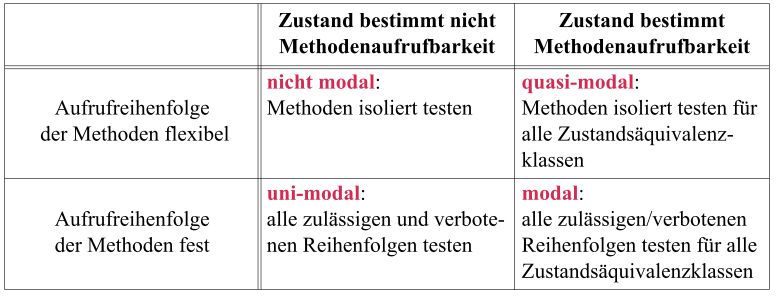
\includegraphics[width=0.85\textwidth]{4_6}
\end{figure}

\paragraph{Vorüberlegungen zur Realisierung von Invarianten,...:}
\begin{itemize}
	\item die teuere Überprüfung von Invarianten, ... muss durch ''Compile''-Flag abschaltbar sein (entweder systemweit oder je Subsystem)
	\item die Überprüfungen dürfen das Verhalten des ausführbaren Programms (abgesehen von Laufzeit und Speicherplatzverbrauch) nicht veränder 
	\item bei abgeschalteten Überprüfungen sollte soweit möglich der Code für diese Überprüfungen nicht Bestandteil des ausführbaren Programms sein
	\item die Reaktion auf fehlgeschlagene Überprüfungen muss an einer Stelle (veränderbar) festgelegt werden (Programmabbruch, Ausnahmeerweckung, ... )
	\item die Überprüfungen sollten möglichst lesbar niedergeschrieben werden
	\item Invarianten werden auch vor der Ausführung einer Methode und nach der Ausführung von ''Observer''-Methoden überprüft (um illegale Objektzugriffe entdecken zu können)
\end{itemize}

\paragraph{Zusicherungen (Assertions) in Java:}
\begin{itemize}
	\item Java besitzt ab Version 1.4 „assert“-Statement, das für den Einbau von Überprüfungen (Vor-/Nachbedingungen, Invarianten) genutzt wird
	\item die Überprüfung von ''assert''-Statements kann durch Runtime-Flags generell oder klassenweise an- bzw. abgeschaltet werden (''-enableassertions'' = ''-ea'' und ''.-disableassertions'' = ''-da'')
	\item die Überprüfungen sollten das Verhalten des ausführbaren Programms (abgesehen von Laufzeit und Speicherplatzverbrauch) nicht verändern (der Programmierer muss das sicherstellen)
	\item soll der Code für ''assert''-Statements nicht Bestandteil des ausführbaren Programms sein, so muss der Compiler davon ''überzeugt'' werden, dass der Code wegoptimiert werden kann
	\item ''assert''-Verletzungen können als ''AssertionError''-Ausnahmen abgefangen werden (und damit im Code festgelegte Reaktionen auslösen)
\end{itemize}

\paragraph{Einsatz von Automaten (Statecharts) zur Testplanung:}

Oft lassen sich die Vorbedingungen für den Aufruf von Methoden besser durch ein Statechart (hierarchischer Automat, siehe Software Eng. - Einführung) darstellen. Ein solches Statechart kann dann - ähnlich wie ein Kontrollflussgraph - zur Planung von Testfällen zur Berechnung von Testüberdeckungsmetriken herangezogen werden.

\begin{figure}[h]
	\centering
	\caption{Einsatz von Automaten (Statecharts) zur Testplanung}
	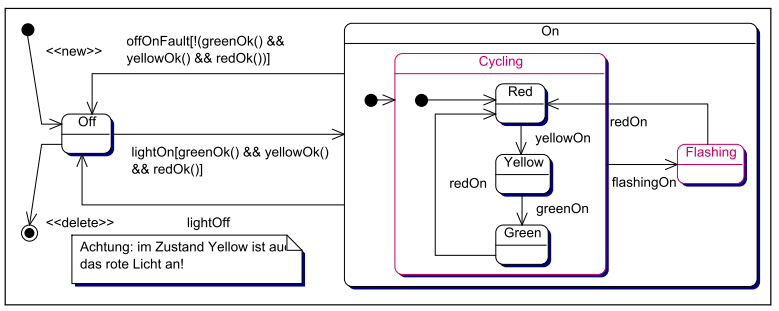
\includegraphics[width=0.85\textwidth]{4_6_1}
\end{figure}

\paragraph{Präzisierung der vier verschiedenen Arten von Klassen:}
\begin{itemize}
	\item Nicht modale Klasse:
	\begin{itemize}
		\item keine Methode der Klasse hat eine Vorbedingung über Attributen
		\item der Zustandsautomat der Klasse besteht aus einem Zustand
	\end{itemize}
	\item Quasimodale Klasse:
	\begin{itemize}
		\item mindestens eine Methode hat eine Vorbedingung über Attributen
		\item der Zustandsautomat der Klasse besteht aus einem Zustand
	\end{itemize}
	\item Unimodale Klasse:
	\begin{itemize}
		\item keine Methode der Klasse hat eine Vorbedingung über Attributen
		\item der Zustandsautomat der Klasse besteht aus mehreren Zuständen
	\end{itemize}
	\item Modale Klasse:
	\begin{itemize}
		\item mindestens eine Methode hat eine Vorbedingung über Attributen
		\item der Zustandsautomat der Klasse besteht aus mehreren Zuständen
	\end{itemize}
\end{itemize}

\paragraph{Definition von Testüberdeckungsmetriken für Statecharts:}
\begin{itemize}
	\item Tests müssen garantieren, dass alle Zustände mindestens einmal erreicht werden
	\item Tests müssen garantieren, dass jede Transition mindestens einmal ausgeführt wird
	\item Tests müssen garantieren, dass jede Transition mit allen sich wesentlich unterscheidenden Belegungen ihrer Bedingung ausgeführt wird
	\item Tests müssen alle möglichen Pfade durch Statechart (bis zu einer vorgegebenen Länge oder vorgegebenen Anzahl von Zyklen) ausführen
	\item zusätzlich zum Test aller explizit aufgeführten Transitionen werden für jeden Zustand alle sonst möglichen Ereignisse (Methodenaufrufe) ausgeführt 
\end{itemize}

\paragraph{Testplanung mit Transitionsbaum (Übergangsbaum) aus [Bi00]:}
\begin{enumerate}
	\item das gegebene Statechart wird in einen flachen Automaten übersetzt
	\item Transitionen mit komplexen Boole’schen Bedingungen werden in mehrere Transitionen mit Konjunktion atomarer Bedingungen übersetzt (Transition mit [(a1 \&\& a2) || (b1 \&\& b2)] wird ersetzt durch Transition mit [a1 \&\& a2] und Transition mit [b1 \&\& b2]
	\item ein Baum wird erzeugt, der
	\begin{itemize}
		\item initialen Zustand als Wurzelknoten (ersten, obersten Knoten) besitzt
		\item Zustandsknoten im Baum werden expandiert, indem alle Transitionen zu anderen Zuständen (und sich selbst) als Kindknoten hinzugefügt werden
		\item jeder Zustand wird nur einmal als Knoten im Transitionsbaum expandiert
	\end{itemize}
	\item jeder Pfad in dem Baum (von Wurzel zu einem Blatt) entspricht einer Testsequenz
	\item zusätzlich werden in jedem Zustand alle Ereignisse ausgelöst, die nicht im Transitionsbaum aufgeführt sind (spezifikationsverletzende Transitionen)
\end{enumerate}

\paragraph{Behandlung ereignisloser Transitionen:}

Automatenmodelle für die Verhaltensbeschreibung wie UML-Statecharts erlauben oft auch die Definition ereignisloser Transitionen. Diese werden wie folgt beim Testen behandelt:


\begin{itemize}
	\item Transition \textbf{ohne Ereignis mit Bedingung} [b]: sobald die Bedingung erfüllt ist, schaltet die Transition; beim Aufstellen von Testsequenzen sind zwei Fälle zu unterscheiden (zwei Unterbäume im Transitionsbaum):
	\begin{itemize}
		\item Bedingung b ist bereits erfüllt, wenn Startzustand der Transition betreten wird (Transition wird mit der Bedingung ''[b == true]'' markiert und schaltet sofort bei der Testausführung)
		\item Bedingung ist nicht erfüllt, wenn Startzustand betreten wird; wird später aber erfüllt (Transition wird mit Ereignis ''b -> true'' markiert und schaltet sobald die Bedingung b erfüllt ist)
	\end{itemize}
	\item Transition \textbf{ohne Ereignis und ohne Bedingung}: die Transition schaltet, sobald der Startzustand betreten wird: der Startzustand erhält im Transitionsbaum eine ausgehende Kante/Transition ohne Markierung
\end{itemize}

\paragraph{Ausführung der Testsequenzen:}
\begin{itemize}
	\item \textbf{Testvorbereitung}: Objekt muss in initialen Zustand (zurück-)versetzt werden
	\item \textbf{Testausführung} einer Sequenz von Methodenaufrufen (Testvektor): es wird unterschieden 
	\begin{itemize}
		\item \textbf{white-box-Sicht}: es gibt Zugriffsoperationen für Abfrage des internen Zustands; man kann also am Ende einer Testsequenz abfragen, ob richtiger Zustand erreicht wurde (interne Zustände der Implementierung müssen mit ''extern'' definierten Zuständen korrespondieren)
		\item \textbf{black-box-Sicht}: Aussenverhalten muss überprüft werden
	\end{itemize}
	\item \textbf{Testbeendigung}: ggf. wird Sequenz von Methodenaufrufen so vervollständigt, dass am Ende der Ausführung Objekt sich in einem ''terminalen'' Zustand befindet
	\item \textbf{Kombination} von Testsequenzen: um Aufwand für Initialisierung zu reduzieren, werden möglichst lange Testsequenzen generiert bzw. kombiniert
\end{itemize}

\paragraph{Abschließende Checkliste für Klassentest nach [Bi00]:}
\begin{itemize}
	\item jede Methode (auch die geerbten) wird mindestens einmal ausgeführt
	\item  alle Methodenparameter und alle nach aussen sichtbaren Attribute werden mit geeigneter Äquivalenzklassenbildung durchgetestet
	\item alle auslösbaren (ausgehenden) Ausnahmen werden mindestens einmal ausgelöst
	\item alle von gerufenen Methoden auslösbaren (eingehenden) Ausnahmen werden mindestens einmal behandelt (oder durchgereicht)
	\item alle identifizierten Objektzustände (auch hier Äquivalenzklassenbildung) werden beim Testen erreicht
	\item jede zustandsabhängige Methode wird in jedem Zustand ausgeführt (auch in den Zuständen, in denen ihr Aufruf nicht zulässig ist)
	\item alle möglichen Zustandsübergänge (mit allen Kombinationen von Bedingungen an den Übergängen) werden aktiviert
	\item zusätzlich werden die üblichen Performanz-, Last-, ... -Tests durchgeführt
\end{itemize}

\subsection{Mutationsbasierte Testverfahren}

\paragraph{Hypothesen}
\begin{itemize}
	\item Programmierer erstellen (oft) annährend korrekte Programme (Competent Programmer Hypothesis)
	\item Komplexe Fehler bedingen häufig die Existenz von simplen Fehlern (Coupling Effect)
\end{itemize}
\paragraph{Schlussfolgerungen}
\begin{itemize}
	\item Typische Programmierfehler lassen sich oft auf kleine syntaktische Änderungen (Mutationen) eines korrekten Programmes zurückführen
	\item Solche Programmmutationen lassen sich automatisiert durchführen
	\item Testfälle sind ''gut'', die bei gleichen Eingaben zu unterschiedlichen Ausgaben (unterschiedlichem Verhalten) eines Programms und eines seiner Mutanten führen
\end{itemize}

\paragraph{Anforderungen an (stark-)mutationserkennende Testfälle}

Der gesuchte Testfall soll bei seiner Ausführung
\begin{itemize}
	\item die fehlerhafte Stelle erreichen (\textbf{Reachability Condition}),
	\item der Programmzustand soll infiziert werden (\textbf{Infection Condition}), also während der Ausführung zu veränderten Variablenbelegungen führen
	\item und der infizierte Programmzustand soll in das Ergebnis propagiert werden (\textbf{Propagation Condition}), dieses also verändern.
\end{itemize}
\textbf{Achtung:}
\begin{itemize}
	\item Ist die ''Propagation Condition'' erfüllt, dann ist auch die ''Infection Condition'' zwangsläufig erfüllt.
	\item Ist die ''Infection Condition'' erfüllt, dann ist auch die ''Reachability Condition'' zwangsläufig erfüllt.
	\item Bislang für die Auswahl von Testfällen benutzte Programmüberdeckungs kriterien konzentrieren sich auf die ''Reachability Conditions''
\end{itemize}

\paragraph{Mutationsbasierte Testsuite-Bewertung:}
\begin{itemize}
	\item gegeben ist ein potentiell fehlerhaftes Programm p und eine \textbf{Test-Suite} TS, die aus einer Menge von Testfällen ${tc1, tc2, ... }$ besteht
	\item zunächst wird eine Menge von \textbf{Mutanten} $M = {m1, m2, ... }$ erzeugt, die sich in der Regel jeweils nur an einer Programmstelle vom Originalprogramm p unterscheiden (Programme mi mit mehreren Unterschieden gegenüber p werden \textbf{Mutanten höherer Ordnung} genannt)
	\item dann werden alle Testfälle der Test-Suite TS auf dem Programm $p$ und der Menge seiner Mutanten $M$ ausgeführt
	\item die Test-Suite bzw. ein Testfall tötet einen Mutanten $m_i$ , falls die Ausführung von $p$ und $m_i$ unterschiedliche Ausgaben erzeugen
	\item \textbf{Effektivität} einer Test-Suite: Anzahl der getöteten Mutanten
	\item \textbf{Effizienz} einer Test-Suite: Anzahl der benötigten Testfälle
	\item Erhöhung der Effizienz einer Test-Suite ohne Reduktion ihrer Effektivität: Testfälle, die keinen Mutanten töten, werden eliminiert; gleiches gilt für Teilmengen von Testfällen, die alle den selben Mutanten töten)
\end{itemize}

\paragraph{Mutationsbasierte Testsuite-Generierung:}

Die werkzeuggestützte Erzeugung von Testfällen, die bestimmte Mutanten töten, ist ein ''schwieriges'' Problem (i.A. nicht berechenbar).

\begin{itemize}
	\item naiver Ansatz: zufallsgesteuerte Erzeugung von Testfällen
	\item verifikationsbasierter Ansatz: das Problem der Erzeugung eines (fehlenden) Testfalles, der einen bestimmten Mutanten m eines Programms p tötet, wird in ein Verifikationsproblem übersetzt:
	\begin{itemize}
		\item erzeugt wird ein neues Programm, das p und m  hintereinander ausführt und die Ausgaben der Ausführung von p und m in verschiedenen Variablen speichert
		\item verifiziert wird dann die Eigenschaft des neuen Programms, für alle möglichen Eingaben bei der Ausführung von p und m immer die gleichen Ausgaben zu produzieren
		\item jedes von einem Verifikationswerkzeug produzierte Gegenbeispiel zu dieser Eigenschaft legt einen Testfall fest, der den Mutanten m tötet
	\end{itemize}
\end{itemize}

\paragraph{Bewertung des Ansatzes [ABL05]:}
\begin{itemize}
	\item Ähnlichkeit zwischen mechanisch erzeugten Mutanten und realen Fehlern ist größer als zwischen manuell eingebauten Fehlern und realen Fehlern
	\item bei manuell eingebauten Fehlern wird die Erkennungsrate einer Test-Suite unterschätzt (manuell eingebaute Fehler sind oft schwerer zu detektieren als mechanisch erzeugte Mutationen)
	\item (ausgewählte) Mutanten sind nicht einfacher oder schwerer zu detektieren als reale Fehler
\end{itemize}

\subsection{Testmanagement und Testwerkzeuge}
Testen wird nach [SL19] immer wie folgt durchgeführt:
\begin{itemize}
	\item \textbf{Testplanung}: es werden die zum Einsatz kommenden Methoden und Werkzeuge sowie die zu testenden Objekte  in einem Testkonzept festgelegt
	\item \textbf{Testüberwachung und Teststeuerung}: Durchführung, Protokollierung und Bewertung der folgenden Aktivitäten inklusive Entscheidung über Testende
	\item \textbf{Testanalyse}: es wird festgelegt was genau zu testen ist durch Überprüfung vorhandener Anforderungspezifikationen, Testobjekte, ...
	\item \textbf{Testentwurf}: es wird festgelegt wie getestet wird; dabei werden abstrakte (mit Bedingungen für Eingabewerte) oder konkrete Testfälle (mit konkreten Eingabewerten) spezifiziert
	\item \textbf{Testrealisierung}: es werden die spezifizierten Testfälle implementiert
	\item \textbf{Testdurchführung}: die ausgewählten Testfälle werden ausgeführt
	\item \textbf{Testabschluss}: es werden die Ergebnisse der vorangegangenen Aktivitäten zusammengetragen und konsolidiert
\end{itemize}

\paragraph{Aufgaben, Qualifikationen und Rollen nach [SL19]:}
\begin{itemize}
	\item \textbf{Testmanager} (Leiter): ist für Management der Testaktivitäten, der Testressourcen und die Bewertung des Testobjekts (gegenüber Projektmanager) verantwortlich
	\item \textbf{Testdesigner} (Analyst): erstellt Testspezifikationen und ermittelt Testdaten [ Ergänzung: könnte beim modellbasierten Testen auch für die Erstellung von Testmodellen und Festlegung von Überdeckungskriterien zuständig sein ]
	\item \textbf{Testfallgenerator}: werden Testfälle aus Modellen bzw. Spezifikationen automatisch erzeugt, so bedarf es einer weiteren Rolle, die die Testfallgenerierung mit Werkzeugunterstützung durchführt
	\item \textbf{Testautomatisierer}: realisiert die automatisierte Durchführung der spezifizierten Testfälle durch ausgewählte Testwerkzeuge
	\item \textbf{Testadministrator}: stellt die Testumgebung mit ausgewählten Testwerkzeugen zur Verfügung (zusammen Systemadministratoren etc.)
	\item \textbf{Tester}: ist für Testdurchführung, -protokollkierung und -auswertung zuständig (entspricht ''Certified Tester Foundation Level''-Kompetenzen) 
\end{itemize}


\paragraph{Weitere Aspekte des Testmanagements nach [SL19]:}
\begin{itemize}
	\item Betrachtung von \textbf{Kosten- und Wirtschaftlichkeitsaspekten}
	\begin{itemize}
		\item Ermittlung und AbschätzunTeststrategieg von Fehlerkosten
		\item Ermittlung und Abschätzung von Testkosten / Testaufwand
	\end{itemize}
	\item Wahl einer \textbf{}
	\begin{itemize}
		\item proaktiv vs. reaktiv (Testmanagement startet mit Projektbeginn vs. Testaktivitäten werden erst nach der Erstellung der Software gestartet)
		\item Testerstellungsansatz / Überdeckungskriterien / ...
		\item Orientierung an Standards für Vorgehensmodelle
	\end{itemize}
	\item Testen und \textbf{Risiko}
	\begin{itemize}
		\item Risiken beim Testen (Ausfall von Personal, ... )
		\item Risikobasiertes Testen (Fokus auf Minimierung von Produktrisiken)
	\end{itemize}
\end{itemize}

\paragraph{Meldung von Fehlern/Fehlermanagement:}
Es müssen alle Informationen erfasst werden, die für das Reproduzieren eines Fehlers notwendig sind. Eine Fehlermeldung kann wie folgt aufgebaut sein:
\begin{itemize}
	\item \textbf{Status}: Bearbeitungsfortschritt der Meldung (Neu, Offen, Analyse, Abgewiesen, Korrektur, Test, Erledigt)
	\item \textbf{Klasse}: Klassifzierung der Schwere des Problems (Menschenleben in Gefahr, Systemabsturz mit Datenverlust, ... , Schönheitsfehler)
	\item \textbf{Priorität}: Festlegung der Dringlichkeit, mit der Fehler behoben werden muss (sofort, da Arbeitsablauf blockiert beim Anwender, ... )
	\item \textbf{Anforderung}: die Stelle(n) in der Anforderungsspezifikation, auf die sich der Fehler bezieht
	\item \textbf{Fehlerquelle}: in welcher Softwareentwicklungsphase wurde der Fehler begangen
	\item \textbf{Fehlerart}: Berechnungsfehler, ...
	\item \textbf{Testfall}: genaue Beschreibung des Testfalls, der Fehler auslöst
	\item ...
\end{itemize}

\paragraph{Arten von Testwerkzeugen:}
Testwerkzeuge werden oft ''\textbf{Computer-Aided Software Test}''-Werkzeuge genannt (\textbf{CAST-Tools}). Man unterscheidet folgene Arten von CAST-Tools:
\begin{itemize}
	\item Werkzeuge zum \textbf{Testmanagement} und zur Testplanung: Erfassen von Testfällen, Abgleich von Testfällen mit Anforderungen, Verwaltung und (statistische) Auswertung von Fehlermeldungen, ...
	\item Werkzeuge zur \textbf{Testspezifikation}: Testdaten und Soll-Werte für zugehörige Ergebnisse werden (manuell) festgelegt und verwaltet
	\item \textbf{Testdatengeneratoren}: aus Softwaremodellen, Code, Grammatiken, ... werden automatisch Testdaten generiert
	\item \textbf{Testtreiber}: passend zu Schnittstellen von Testobjekten werden Testtreiber bzw. Testrahmen zur Verfügung gestellt, die die Aufruf von Tests mit Übergabe von Eingabewerten, Auswertung der Ergebnisse etc. abwickeln
	\item \textbf{Simulatoren}: bilden möglichst realitätsnah Produktionsumgebung nach (mit Simulation von anderen Systemen, Hardware, ... )
	\item \textbf{Testroboter} (Capture \& Replay-Werkzeug): zeichnet interaktive Benutzung einer Bedienungsoberfläche auf und kann Dialog wieder abspielen (solange sich Oberfläche nicht zu stark verändert)
	\item Werkzeuge für Last- und \textbf{Performanztests} (dynamische Analysen): Laufzeitmessungen, Speicherplatzverbrauch, ...
	\item \textbf{Komparatoren}: vergleichen erwartete mit tatsächlichen Ergebnissen, filtern unwesentliche Details, können ggf. auch Zustand von Benutzeroberflächen prüfen
	\item \textbf{Code-Überdeckungsanalysatoren}: für gewählte Überdeckungsmetriken wird Buch darüber geführt, wieviel Prozent Überdeckung erreicht ist, welche Programmausschnitte noch nicht überdeckt sind
	\item Werkzeuge für \textbf{statische Analysen}: Berechnung von Metriken, Kontroll- und Datenflussanomalien, ...
\end{itemize}

\subsection{Zusammenfassung}
Dynamische Programmanalysen und das ''traditionelle'' Testen sind die wichtigsten Mittel der analytischen Qualitätssicherung. Mindestens folgende Maßnahmen sollten immer durchgeführt werden:
\begin{itemize}
	\item Suche nach Speicherlecks und Zugriff auf nichtinitialisierte Speicherbereiche (oder falsche Speicherbereiche) mit geeigneten Werkzeugen
	\item automatische Regressions-Testdurchführung mit entsprechenden Frameworks zur Testautomatisierung
	\item Überprüfung der Zweigüberdeckung durch Testfälle anhand von Kontrollflussgraph (durch Werkzeuge)
	\item Verwendung von ''Black-Box''-Testverfahren mit Äquivalenzklassenbildung für Eingabeparameter (Objekte) zur Bestimmung von Testfällen
	\item Einbau möglichst vieler abschaltbarer Konsistenzprüfungen in Code (Vor- und Nachbedingungen) und ggf. defensive Programmierung
\end{itemize}




